\chapter{El Sol en el cielo: los días y las estaciones}\label{ch:g3:sun-days-seasons}

En junio juegas fuera después de cenar con una \omterm{def:g1:light-and-shadows:source}{luz} dorada; en
diciembre las farolas se encienden antes de que vuelvas del colegio.
El Sol conserva su vieja costumbre --- sube por un lado, pasa por lo
más alto y baja por el otro ---, pero su camino por el cielo no es el
mismo durante todo el año. Síguelo un año entero y descubrirás las
\omterm{def:g3:sun-days-seasons:year}{estaciones}.

\section{El camino cambiante del Sol}

\begin{example}[Camino de verano, camino de invierno]\label{ex:g3:sun-days-seasons:roads}
Observa el arco del Sol en pleno verano: sale pronto, sube muy alto
--- casi encima de tu cabeza al mediodía --- y se pone tarde: un
camino largo y alto, y un día largo. En pleno invierno, el arco es
bajo y corto: el Sol sale tarde, no llega a subir mucho por encima de
los tejados y se pone a media tarde. Entre los dos, en primavera y en
otoño, el camino es intermedio --- y el día y la noche se reparten las
\omterm{ex:g2:measuring-time:clock}{horas} casi por igual.
\end{example}

\begin{omfigure}
\begin{tikzpicture}[scale=0.85]
  \draw[thick] (0,0) -- (11,0);
  \draw[dashed, omThm, thick] (1.0,0.2) .. controls (3.5,4.6)
    and (7.5,4.6) .. (10.0,0.2);
  \fill[omThm] (5.5,3.5) circle (0.3);
  \node[above, font=\small, omThm] at (5.5,3.9) {pleno verano: alto y largo};
  \draw[dashed, omDef, thick] (2.6,0.15) .. controls (4.4,1.7)
    and (6.6,1.7) .. (8.4,0.15);
  \fill[omDef] (5.5,1.3) circle (0.3);
  \node[above, font=\small, omDef] at (2.9,1.35) {pleno invierno: bajo y corto};
\end{tikzpicture}

{\small Los dos caminos extremos del Sol sobre el mismo horizonte. El
arco alto del verano tarda muchas \omterm{ex:g2:measuring-time:clock}{horas} en recorrerse; el arco bajo
del invierno está terminado a media tarde.}
\end{omfigure}

\begin{proposition}[La regla del mediodía]\label{prop:g3:sun-days-seasons:midday}
En todas las \omterm{def:g3:sun-days-seasons:year}{estaciones}, el Sol está en su punto más alto a mitad
del día --- y en ese instante todas las \omterm{def:g1:light-and-shadows:shadow}{sombras} son lo más cortas del
día y apuntan en la misma dirección que la \omterm{def:g1:light-and-shadows:shadow}{sombra} del mediodía de
ayer y que la de mañana. Las \omterm{def:g1:light-and-shadows:shadow}{sombras} del mediodía son las flechas
más fiables de la naturaleza.
\end{proposition}

\begin{example}[Leer la estación en una sombra]\label{ex:g3:sun-days-seasons:shadowlength}
La \emph{longitud} de la \omterm{def:g1:light-and-shadows:shadow}{sombra} del mediodía cambia con la
\omterm{def:g3:sun-days-seasons:year}{estación}: en verano, con el Sol casi encima de la cabeza, la
\omterm{def:g1:light-and-shadows:shadow}{sombra} de un poste al mediodía es un muñón corto; en invierno, con el
Sol colgando bajo, ese mismo poste echa una \omterm{def:g1:light-and-shadows:shadow}{sombra} larga al mediodía.
Marca en el suelo la punta de la \omterm{def:g1:light-and-shadows:shadow}{sombra} del mediodía una vez al mes y
las marcas irán y vendrán a lo largo del año como un péndulo lento.
\end{example}

\section{El reloj de sombra}

\begin{definition}[Reloj de sol]\label{def:g3:sun-days-seasons:sundial}
Un \emph{reloj de sol}\index{reloj de sol} es un reloj hecho de
\omterm{def:g1:light-and-shadows:shadow}{sombra}: un palo o una lámina plantados al sol, con marcas
alrededor que enseñan dónde cae la \omterm{def:g1:light-and-shadows:shadow}{sombra} a cada hora. Mientras el Sol
recorre su arco, la \omterm{def:g1:light-and-shadows:shadow}{sombra} barre las marcas --- despacio, en silencio
y sin una sola pieza móvil.
\end{definition}

\begin{method}[Construir un reloj de sombra]\label{met:g3:sun-days-seasons:build}
Una mañana soleada, en un sitio que esté al sol todo el día:
\begin{enumerate}
  \item planta un palo recto de pie en un suelo plano (o mételo en un
        cubo de arena);
  \item cada hora, en punto, marca la punta de su \omterm{def:g1:light-and-shadows:shadow}{sombra} con un
        guijarro y escribe la hora en el guijarro con tiza;
  \item sigue así hasta el anochecer.
\end{enumerate}
Mañana, la \omterm{def:g1:light-and-shadows:shadow}{sombra} visitará tus guijarros puntualmente: tu palo ya da
la hora. (Durante una temporada, al menos --- según se desliza la
\omterm{def:g3:sun-days-seasons:year}{estación}, las \omterm{def:g1:light-and-shadows:shadow}{sombras} se deslizan también, y tus guijarros irán
quedándose poco a poco equivocados.)
\end{method}

\begin{omfigure}
\begin{tikzpicture}[scale=0.85]
  \draw[thick] (0.5,0) -- (10.5,0);
  \draw[very thick] (5.5,0) -- (5.5,1.7);
  \draw[line width=3pt, omExo] (5.5,0) -- (2.2,0.9);
  \draw[line width=3pt, omExo, opacity=0.6] (5.5,0) -- (4.1,1.35);
  \draw[line width=3pt, omExo, opacity=0.35] (5.5,0) -- (5.5,1.5);
  \draw[line width=3pt, omExo, opacity=0.6] (5.5,0) -- (6.9,1.35);
  \draw[line width=3pt, omExo] (5.5,0) -- (8.8,0.9);
  \node[font=\footnotesize] at (1.8,1.0) {mañana};
  \node[font=\footnotesize] at (5.5,1.9) {mediodía: la más corta};
  \node[font=\footnotesize] at (9.4,1.0) {tarde};
\end{tikzpicture}

{\small Un palo, un día: la \omterm{def:g1:light-and-shadows:shadow}{sombra} barre el suelo como una aguja
lenta, larguísima en los extremos del día y cortísima al mediodía.}
\end{omfigure}

\section{El año y sus estaciones}

\begin{definition}[El año y las estaciones]\label{def:g3:sun-days-seasons:year}
Mientras la Tierra gira una vez al día, recorre también un viaje
enorme \emph{alrededor del Sol} --- una vuelta completa dura un
\emph{año}\index{año}, unos $365$ días. A lo largo de esa vuelta, el
camino del Sol por nuestro cielo sube y baja despacio, y nosotros
pasamos por las cuatro \emph{estaciones}\index{estación}: primavera,
verano, otoño e invierno --- y otra vez primavera, vuelta tras vuelta.
\end{definition}

\begin{example}[Los cuatro cuartos]\label{ex:g3:sun-days-seasons:quarters}
Verano: Sol alto, días largos, \omterm{def:g1:light-and-shadows:shadow}{sombras} cortas al mediodía. Invierno:
Sol bajo, días cortos, \omterm{def:g1:light-and-shadows:shadow}{sombras} largas al mediodía. La primavera y el
otoño quedan en medio --- y en cada uno de ellos llega un día especial
en el que el día y la noche duran lo mismo. Los campesinos, los
marineros y los constructores de antaño aprendieron a leer este
calendario directamente en el cielo.
\end{example}

\begin{omfigure}
\begin{tikzpicture}[scale=0.85]
  \fill[omThm] (5.5,1.8) circle (0.5);
  \foreach \a in {0,30,...,330} {
    \draw[omThm] (5.5,1.8) ++(\a:0.68) -- ++(\a:0.26);
  }
  \draw[dashed, thick] (5.5,1.8) ellipse (4.4 and 1.55);
  \fill[omDef] (1.1,1.8) circle (0.26);
  \fill[omDef] (9.9,1.8) circle (0.26);
  \fill[omDef] (5.5,3.35) circle (0.26);
  \fill[omDef] (5.5,0.25) circle (0.26);
  \node[left, font=\small] at (0.75,1.8) {aquí, invierno};
  \node[right, font=\small] at (10.25,1.8) {aquí, verano};
  \node[above, font=\small] at (5.5,3.7) {primavera};
  \node[below, font=\small] at (5.5,-0.1) {otoño};
\end{tikzpicture}

{\small Una vuelta de la Tierra alrededor del Sol --- un año, cuatro
\omterm{def:g3:sun-days-seasons:year}{estaciones}. ¿Y por qué el camino bajo en invierno y el alto en
verano? Ese secreto se guarda para un capítulo posterior sobre la
familia Sol--Tierra--Luna.}
\end{omfigure}

\begin{remark}[El invierno no es estar ``más lejos'']\label{rem:g3:sun-days-seasons:notfarther}
Es tentador suponer que en invierno hace frío porque la Tierra se
aleja del Sol. Pues no --- la distancia apenas cambia y, cuando aquí
es invierno, para los niños de la otra mitad de la Tierra es verano en
ese mismísimo instante, ¡algo que ningún ``estar más lejos'' podría
explicar! La clave de verdad es el \emph{camino bajo} del Sol: Sol
bajo, \omterm{def:g1:light-and-shadows:source}{luz} de refilón, poco calentamiento. La explicación completa
queda prometida para un capítulo posterior.
\end{remark}

\begin{omfigure}
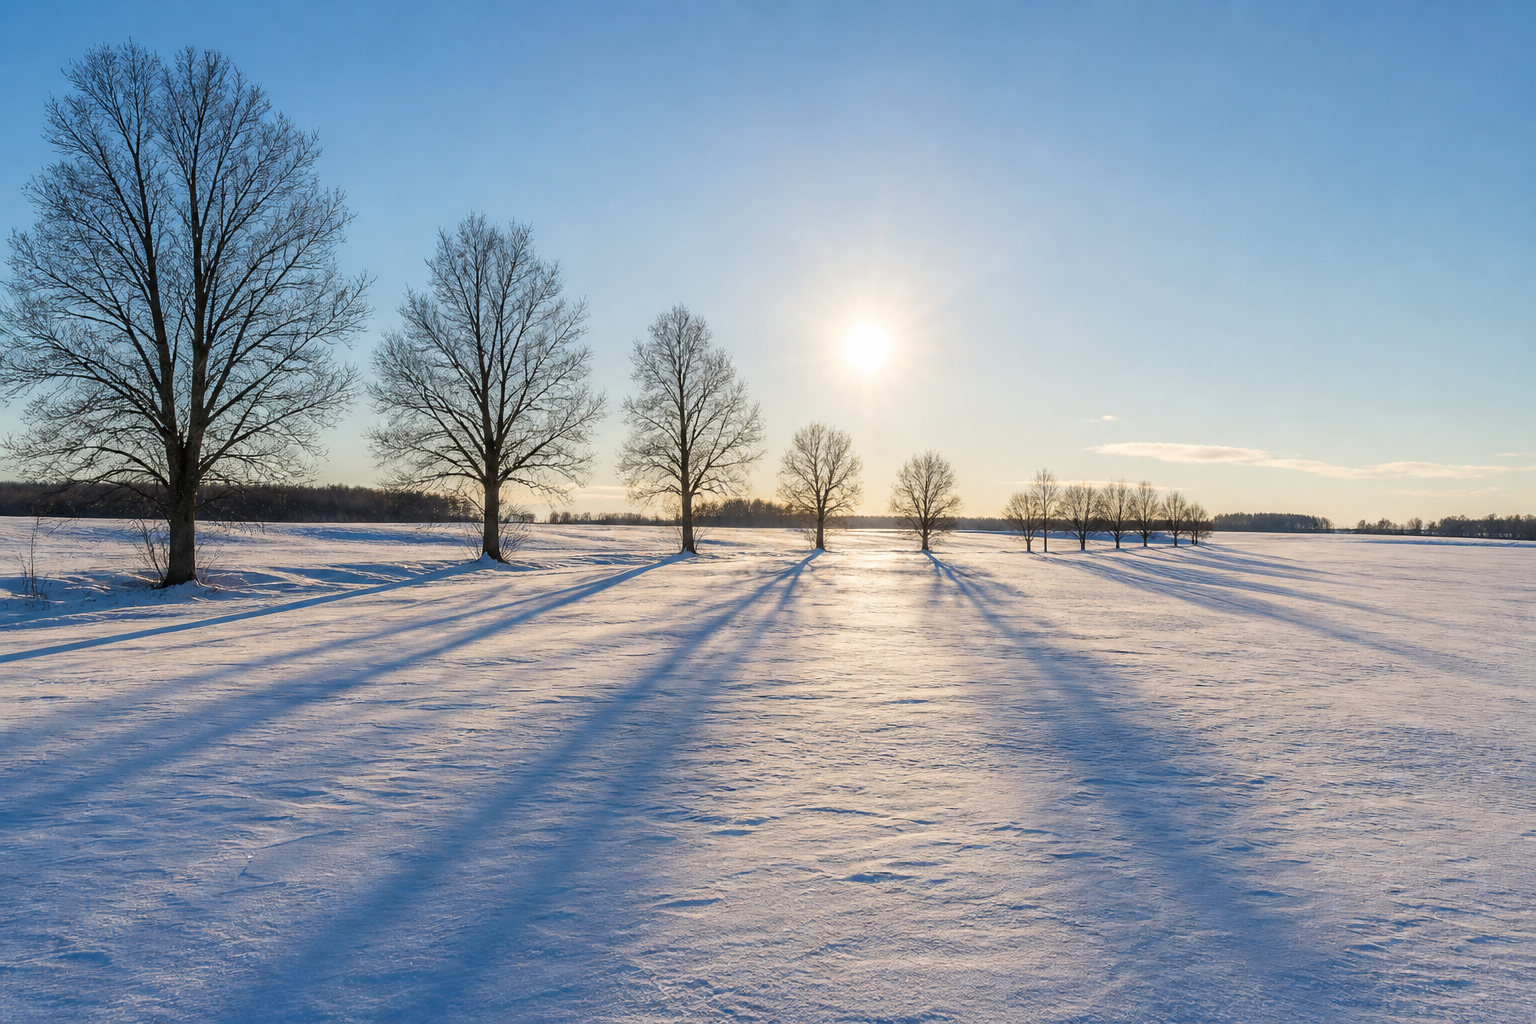
\includegraphics[width=0.58\linewidth]{images/book1/ai/g3-seasons-winter-sun.png}

{\small Un mediodía de invierno: el Sol se queda bajo, la \omterm{def:g1:light-and-shadows:source}{luz} llega de refilón y las \omterm{def:g1:light-and-shadows:shadow}{sombras} se estiran largas sobre la nieve.}
\end{omfigure}

\section{Ejercicios}

\begin{exercise}[$\star$]\label{exo:g3:sun-days-seasons:1}
¿En qué \omterm{def:g3:sun-days-seasons:year}{estación} es el arco del Sol el más alto y el más largo? ¿Y
el más bajo y el más corto? ¿Qué le hace eso a la \omterm{def:g2:measuring-time:duration}{duración} del día?
\end{exercise}

\begin{exercise}[$\star$]\label{exo:g3:sun-days-seasons:2}
¿En qué momento del día es más corta la \omterm{def:g1:light-and-shadows:shadow}{sombra} de un poste? ¿Qué otra
cosa tiene de especial la \omterm{def:g1:light-and-shadows:shadow}{sombra} del mediodía, día tras día?
\end{exercise}

\begin{exercise}[$\star$]\label{exo:g3:sun-days-seasons:3}
El mismo poste echa al mediodía una \omterm{def:g1:light-and-shadows:shadow}{sombra} de $2$ botas de largo en
junio y de $7$ botas en diciembre. Explica la diferencia con los dos
caminos del Sol.
\end{exercise}

\begin{exercise}[$\star$]\label{exo:g3:sun-days-seasons:4}
¿Cómo da la hora un \omterm{def:g3:sun-days-seasons:sundial}{reloj de sol}? ¿De qué está hecha su aguja móvil?
\end{exercise}

\begin{exercise}[$\star$]\label{exo:g3:sun-days-seasons:5}
En el \cref{met:g3:sun-days-seasons:build}, ¿por qué tiene que estar
el palo en un sitio que reciba sol todo el día? ¿Qué le pasa al reloj
cuando está nublado? ¿Y de noche?
\end{exercise}

\begin{exercise}[$\star$]\label{exo:g3:sun-days-seasons:6}
¿Cuánto tarda la Tierra en dar una vuelta alrededor del Sol? ¿Cuántas
\omterm{def:g3:sun-days-seasons:year}{estaciones} caben en una vuelta? Ponlas en orden, empezando por la
primavera.
\end{exercise}

\begin{exercise}[$\star$]\label{exo:g3:sun-days-seasons:7}
¿Cuántos días tiene aproximadamente un año? Y --- de un capítulo
anterior --- ¿cuántas \omterm{ex:g2:measuring-time:clock}{horas} tiene un día? ¿Qué viaje de la Tierra
produce cada uno?
\end{exercise}

\begin{exercise}[$\star$]\label{exo:g3:sun-days-seasons:8}
Nombra dos pistas, visibles desde tu ventana en una sola semana, que
te digan si estás en pleno verano o en pleno invierno sin mirar un
calendario.
\end{exercise}

\begin{exercise}[$\star$]\label{exo:g3:sun-days-seasons:9}
Cuando en tu casa es invierno, ¿qué \omterm{def:g3:sun-days-seasons:year}{estación} es para los niños de la
otra mitad de la Tierra? ¿Qué demuestra esto sobre la suposición ``en
invierno hace frío porque toda la Tierra está más lejos del Sol''?
\end{exercise}

\begin{exercise}[$\star\star$]\label{exo:g3:sun-days-seasons:10}
Una jardinera coloca los guijarros de su reloj de \omterm{def:g1:light-and-shadows:shadow}{sombra} en marzo. En
junio, la \omterm{def:g1:light-and-shadows:shadow}{sombra} ya no toca los guijarros a las \omterm{ex:g2:measuring-time:clock}{horas} marcadas.
¿Se ha movido el palo? Explica qué se ha desplazado, usando el
\cref{ex:g3:sun-days-seasons:shadowlength}.
\end{exercise}

\begin{exercise}[$\star\star$]\label{exo:g3:sun-days-seasons:11}
Una exploradora se despierta sin reloj ni teléfono, ve el Sol
exactamente en su punto más alto y, una hora después, descubre que la
\omterm{def:g1:light-and-shadows:shadow}{sombra} de su tienda ya es más larga que la altura de la tienda.
¿Qué hora era más o menos cuando se despertó y está más cerca del
pleno verano o del pleno invierno? Razónalo con la regla del mediodía
y con la longitud de la \omterm{def:g1:light-and-shadows:shadow}{sombra}.
\end{exercise}
